\section{Solar Coordinates}
\label{sec:coords}

The \package{sunpy.coordinates} subpackage provides:
\begin{itemize}
    \item A robust framework for working with coordinate systems
    \item Functions to obtain the locations of solar-system bodies
    \item Functions to calculate Sun-specific coordinate information
\end{itemize}
The currently supported Sun-centered coordinate systems are Heliocentric Aries Ecliptic (HAE), Heliocentric Cartesian (HCC), Heliocentric Earth Equatorial (HEEQ), Heliographic Carrington (HGC), Heliographic Stonyhurst (HGS), and Helioprojective Cartesian (HPC) \citep[see][]{2006A&A...449..791T}.
Additional coordinate systems are in the process of being implemented and will become available in future releases of the \sunpypkg.
The coordinates framework leverages the \package{astropy.coordinates} subpackage and its \code{SkyCoord} class \citep[see Section 3.3 of][]{astropy2018} by defining the above frames and the transformations between those frames.
A \code{SkyCoord} object specifies both the coordinate frame (e.g., HCC) and a representation of the particular coordinate (e.g., Cartesian coordinates).
Since most frames evolve over time, the \code{SkyCoord} object may also specify the observation time.

The observer-independent coordinate frames -- HAE, HEEQ, HGC, and HGS -- are useful for specifying the locations of features on the Sun or objects (e.g., spacecraft) in interplanetary space.
The commonly used HGS frame is of particular note because it transforms in a straightforward manner to and from the Heliocentric Celestial Reference System (HCRS).
The transformation is the combination of two rotation angles: the time-independent angle between the Sun's rotation axis and the HCRS celestial pole \citep[see][]{2007CeMDA..98..155S} and the time-dependent angle of the central meridian (as seen from Earth) relative to the vernal equinox.
This transformation between HGS and HCRS links the frames defined in \package{sunpy.coordinates} with the the frames defined in \package{astropy.coordinates}, allowing any solar frame to be transformed to and from any astronomical frame (\autoref{fig:transform_graph}).
In fact, HAE is actually implemented in \package{astropy.coordinates} (as \code{HeliocentricMeanEcliptic}), but the shared framework means that it can be used seamlessly in \sunpypkg.

\begin{figure}
    \centering
    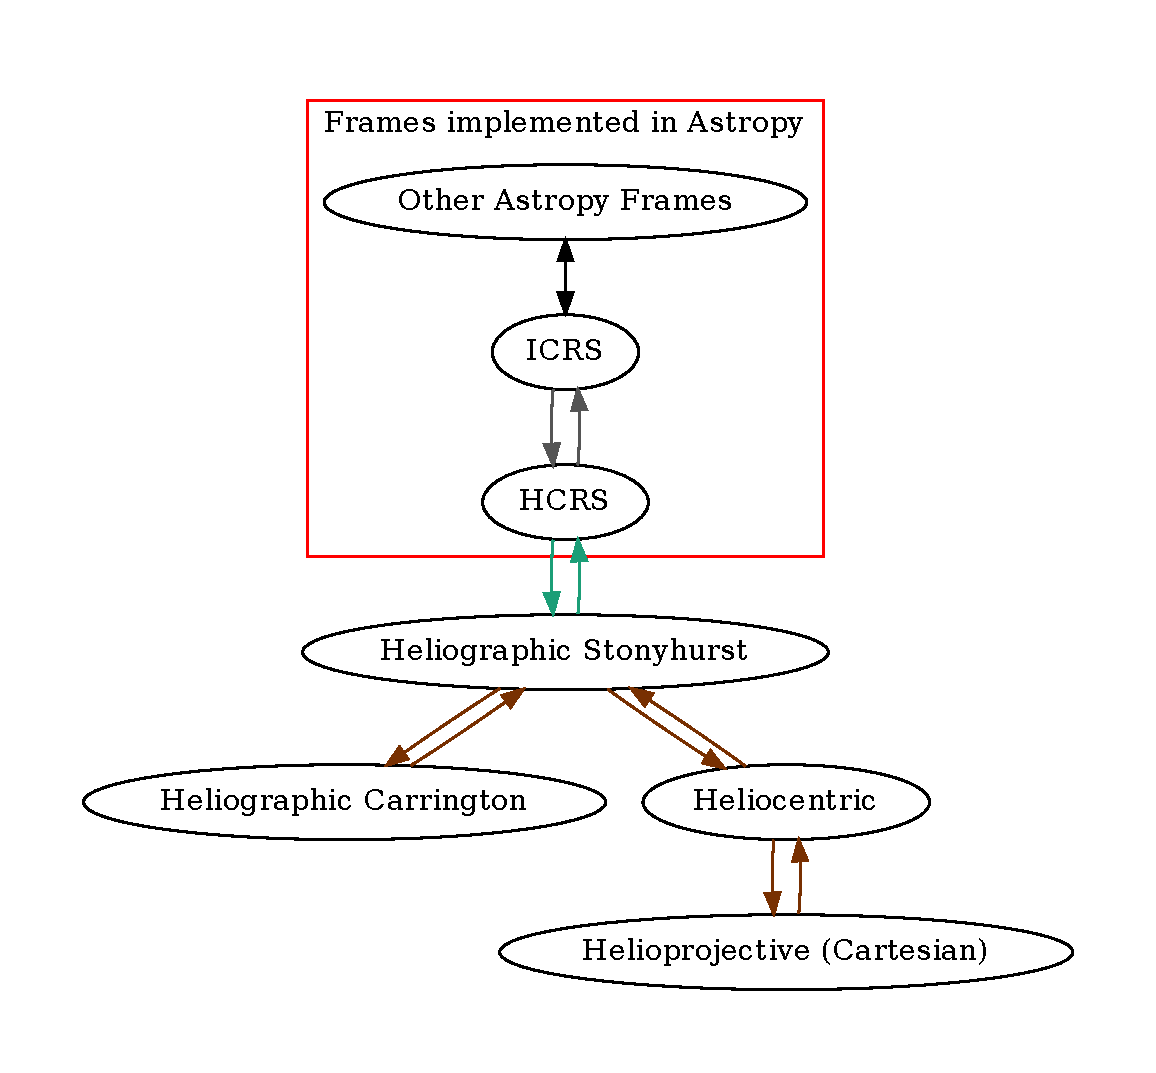
\includegraphics[width=0.75\textwidth]{figures/sunpy_frames.pdf}
    \caption{Graph of the coordinate frames accessible through \package{sunpy.coordinates}, and how they transform between each other.
    The frames within the blue box are actually implemented in \package{astropy.coordinates}, but in the shared framework, any frame can be transformed to any other frame in this graph.}
    \label{fig:transform_graph}
\end{figure}

The observer-dependent coordinate frames -- HCC and HPC -- are useful for observational data, with the potential for subsequent transformation to an observer-independent frame.
The HPC frame in particular is widely used for images from solar missions.
These frames have axes that change orientation depending on the location of the observer, and thus the observer location is necessary to fully define the frame.
This observer location is also stored in the \code{SkyCoord} object.
If the observer is not explicitly specified, the observer is assumed to be at Earth, which may be an adequate approximation for most observations.
Be aware that using the default observer of Earth does not fully define the frame unless the observation time is specified, since the location of Earth needs to be known.

\begin{figure}
    \gridline{\fig{figures/fig_fieldlines_aia.pdf}{0.3\textwidth}{(a)}
              \fig{figures/fig_venus_transit.pdf}{0.3\textwidth}{(b)}
              \fig{figures/fig_coronagraph_starfield.pdf}{0.3\textwidth}{(c)}
              }
    \caption{Several example use cases of the coordinates machinery in \sunpypkg.
    (a) Field lines traced from a potential field extrapolation overlaid on a 171 \AA{} AIA observation of an active region from 2019 March 10 00:00:04 UTC.
    The field extrapolation was computed with \package{pfsspy} \citep{david_stansby_2019_3237053}.
    (b) The Venus transit as viewed by SDO/AIA in 1600 \AA. The predicted position of Venus is overplotted in the helioprojective coordinate frame of the AIA image.
    (c) A coronagraph image of the solar corona as observed by STEREO-A COR-2. The predicted positions of stars from the Gaia DR2 catalog as well as Mars are overplotted.}
    \label{fig:coordinates_examples}
\end{figure}

The \package{sunpy.coordinates} subpackage enables significant functionality in the \sunpycode{Map} object (see \autoref{sec:map}), and a few examples are shown in \autoref{fig:coordinates_examples}.
The center and rightmost panels of \autoref{fig:coordinates_examples} make use of functions in \package{sunpy.coordinates} to obtain the location of solar-system bodies.
\code{get\_body\_heliographic\_stonyhurst} not only returns the location of one of the planets, but can appropriately correct for light travel time to an observer to return the apparent location (in the past) of that planet.
This planet location is obtained using the active ephemeris in \package{astropy.coordinates}, so if one wants the location of a non-Earth body and accuracy is important, one should use \code{astropy.coordinates.solar\_system\_ephemeris} to specify a JPL ephemeris rather than Astropy's default ephemeris.
\code{get\_horizons\_coord} allows one to query JPL HORIZONS\footnote{\url{https://ssd.jpl.nasa.gov/?horizon}} for the location of a wide range of solar-system bodies.
JPL HORIZONS includes ephemeris information not only for planets and other natural bodies in the solar system, but also for major spacecraft such as SDO and SOHO.

The coordinate framework is also used to calculate Sun-specific coordinate information with high accuracy.
These functions are under \package{sunpy.coordinates.sun} and return values such as Carrington rotation number for the provided time.
Nearly all of the returned values match values in the \textit{Astronomical Almanac} to published precision (e.g., the hundredth of an arcsecond for apparent right ascension).
For times that are provided to these functions, one should take care to specify whether the time scale is UTC or some other time scale (see \autoref{sec:units}).

\subsection{Differential Rotation}
\label{sec:differential_rotation}

%1-2 sentences intro; 1-2 sentences describing what is new; 1 sentence that acknowledges the figure.

% Can delete the first two sentences if the background info feels unnecessary

When analyzing the dynamics of observed solar emission, it is important to account for variations due to the rotation of the Sun.
In particular, one must account for \textit{differential rotation}, or the latitudinally-varying rotation rate due to the non-rigidity of the solar interior.
The \package{sunpy.physics.differential\_rotation} subpackage provides tools for transforming both \code{SkyCoord} coordinate and \code{Map} objects according to the differential rotation of the Sun.
The amount of rotation can be specified using either a new time, a time interval, or a new observer location.

While earlier versions of \sunpypkg included tools for dealing with differential rotation, this release includes several improvements.
For example, applying the effect of solar differential rotation now properly accounts for the changing position of the observer.
This can be important because, for example, observers on the Earth must take into account the motion of the Earth in addition to solar differential rotation when calculating how much a location on the Sun appears to move.
\autoref{fig:diff_rot} shows an example using a 1600 \AA{} AIA observation of how differential rotation can be applied to \code{Map} objects.
The image in the middle panel was observed approximately two days after the image in the top panel.
The bottom panel shows the top panel differentially rotated using the observer location and time from the middle panel, showing the good agreement with the actual observation in the middle panel.

\begin{figure}
    \center
    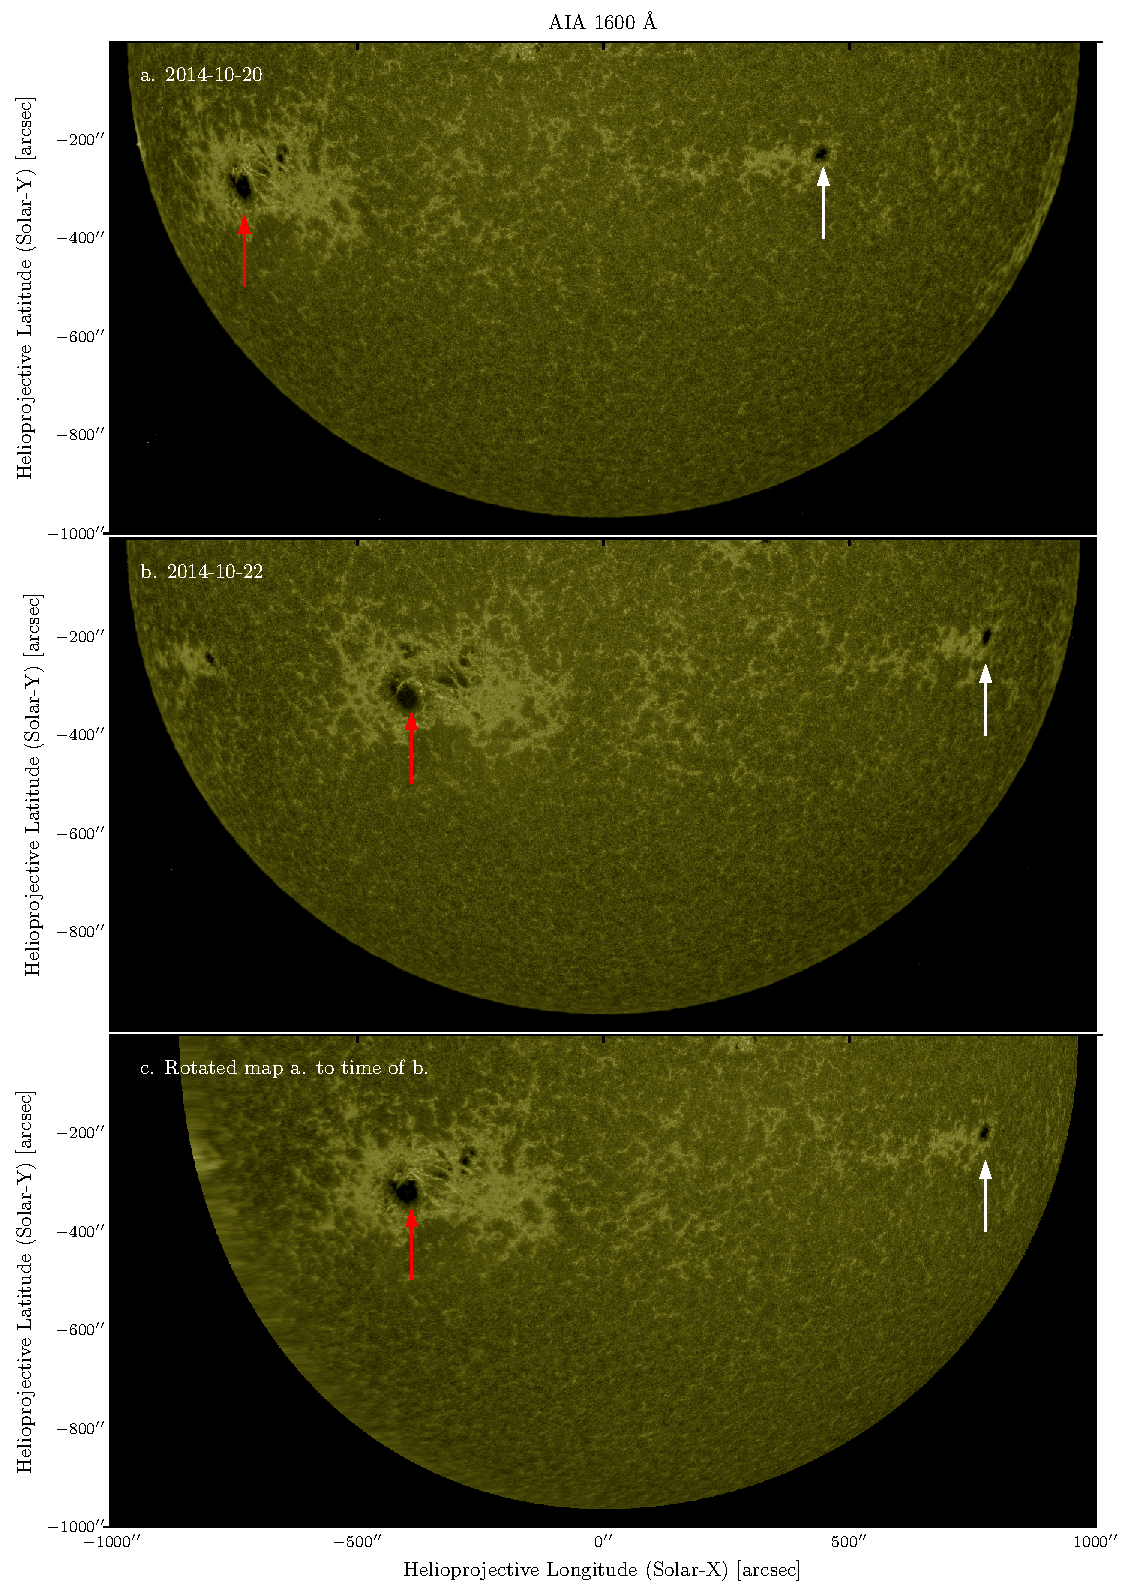
\includegraphics[width = 0.8\textwidth]{figures/fig_diff_rot_1600.pdf}
    \caption{Example of the functionality of \sunpypkg to apply solar differential rotation to a Map.
    Panels (a) and (b) show the Sun as observed in AIA 1600~\AA\ on two different days, 2014-02-20 and 2014-02-22.
    A large sunspot group is highlighted by the red arrow, and a smaller sunspot by the white arrow.
    Panel (c) shows the map of (a) that has been rotated differentially using \sunpypkg to the time of map (b).}
    \label{fig:diff_rot}
\end{figure}
